\documentclass[11pt]{article}

\usepackage[utf8]{inputenc}
\usepackage[margin=1in]{geometry} 
\usepackage{amsmath,amsthm,amssymb,graphicx,mathtools,tikz,hyperref,multicol,cancel,enumitem,booktabs,float,pgfplots,multirow,mathrsfs,textcomp,gensymb,soul,changepage,threeparttable}
%\usepackage[table]{xcolor}
\usepackage[T1]{fontenc}
\usepackage[italian]{babel}
\usepackage{hyphenat}
\hyphenation{mate-mati-ca recu-perare}
\usetikzlibrary{positioning}
\pgfplotsset{compat=1.14}

\newcommand{\n}{\mathbb{N}}
\newcommand{\z}{\mathbb{Z}}
\newcommand{\q}{\mathbb{Q}}
\newcommand{\cx}{\mathbb{C}}
\newcommand{\real}{\mathbb{R}}
\newcommand{\field}{\mathbb{F}}
\newcommand{\ita}[1]{\textit{#1}}
\newcommand{\com}[2]{#1\backslash#2}
\newcommand{\oneton}{\{1,2,3,...,n\}}
\newcommand{\idea}[1]{\begin{gather*}#1\end{gather*}}
\newcommand{\ef}{\ita{f} }
\newcommand{\eff}{\ita{f}}
\newcommand{\proofs}[1]{\begin{proof}#1\end{proof}}
\newcommand{\inv}[1]{#1^{-1}}
\newcommand{\setb}[1]{\{#1\}}
\newcommand{\en}{\ita{n }}
\newcommand{\vbrack}[1]{\langle #1\rangle}
\newcommand{\qRa}{\quad \Rightarrow \quad}
\newcommand{\smaca}[1]{\textbf{\textsc{#1}}}

\newenvironment{theorem}[2][Teorema]{\begin{trivlist}
\item[\hskip \labelsep {\bfseries #1}\hskip \labelsep {\bfseries #2.}]}{\end{trivlist}}
\newenvironment{lemma}[2][Lemma]{\begin{trivlist}
\item[\hskip \labelsep {\bfseries #1}\hskip \labelsep {\bfseries #2.}]}{\end{trivlist}}
\newenvironment{exercise}[2][Esercizio]{\begin{trivlist}
\item[\hskip \labelsep {\bfseries #1}\hskip \labelsep {\bfseries #2.}]}{\end{trivlist}}
\newenvironment{proposition}[2][Proposizione]{\begin{trivlist}
\item[\hskip \labelsep {\bfseries #1}\hskip \labelsep {\bfseries #2.}]}{\end{trivlist}}
\newenvironment{corollary}[2][Corollario]{\begin{trivlist}
\item[\hskip \labelsep {\bfseries #1}\hskip \labelsep {\bfseries #2.}]}{\end{trivlist}}

\hypersetup {
    colorlinks,
    linkcolor=blue
}

\graphicspath{{img/}}

\begin{document}
\setlength{\parindent}{0pt}
\title{\vspace{-4em}{\large Laboratorio di Meccanica e Termodinamica} \\
    Relazione di Laboratorio}
\author{Gerardo Selce, Maurizio Liguori, Emanuela, Francesco Messano}
\date{22 Ottobre 2024}
\maketitle


\vspace{-2em}\par\noindent\rule{\textwidth}{0.4pt}
\begin{center}
    {\Large\sc Misura della densità di un solido}
\end{center}
\par\noindent\rule{\textwidth}{0.4pt}
\section{Scopo dell'esperienza}
Lo scopo dell’esperienza consiste nella stima della densità di tre diversi corpi solidi, confrontando il risultato ottenuto con le densità di alcuni materiali noti e infine usare questa informazione per capire di quale materiale è composto ogni solido analizzato.
I tre corpi solidi sono cilindri di diverse dimensioni.
Per poter ottenere la densità di ciascuno di essi abbiamo dovuto misurare sia il volume che la massa di ognuno.

\section{Richiami teorici}
La densità di un corpo è una costante propria di ogni materiale definita come la quantità di massa contenuta in un dato volume. Operativamente è definibile come il rapporto tra la massa e il volume: \begin{displaymath}
\rho=\frac{m}{V}\
\end{displaymath}


\section{Descrizione dell'apparato sperimentale}
Per misurare le grandezze lineari che intervengono nella definizione di volume è stato usato un calibro a corsoio con nonio.

\begin{figure}[ht]
  \centering
  \includegraphics[width=0.5\textwidth]{IMG_0205.pdf}
  \caption{Calibro utilizzato in laboratorio}
\end{figure}

Il calibro a corsoio con nonio cinquantesimale è uno strumento di misura di precisione utilizzato per determinare dimensioni lineari, come lunghezze, diametri e profondità. È dotato di un nonio con una scala che permette letture fino a 0,02 mm, consentendo misurazioni molto accurate. La scala principale e il nonio scorrono l'una rispetto all'altra per effettuare la lettura della misura finale.

Per misurare la massa dei cilindri è stata utilizzata una bilancia digitale con risoluzione al centesimo di grammo e con portata di 820g.

\begin{figure}[ht]
  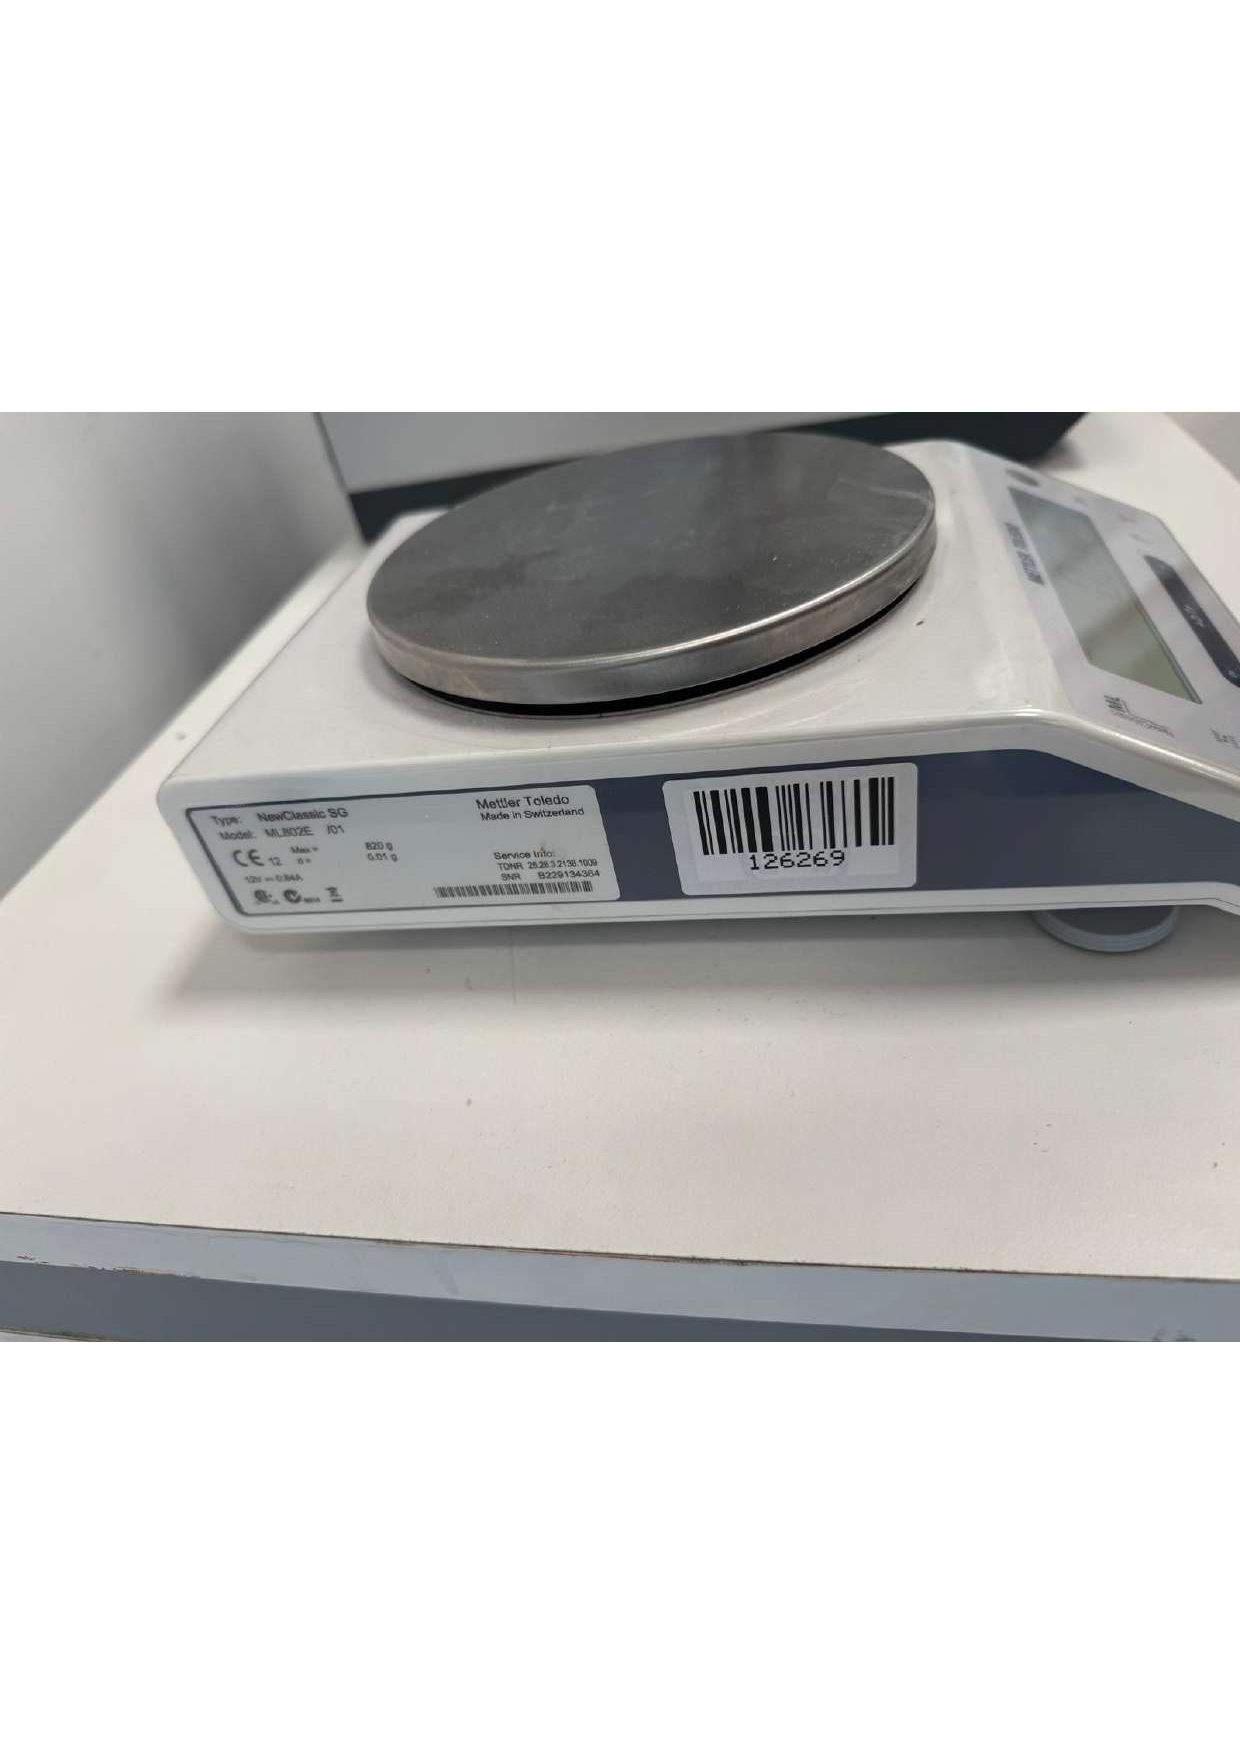
\includegraphics[width=0.5\textwidth]{WhatsApp Image 2024-10-25 at 16.42.15 (1).pdf}
  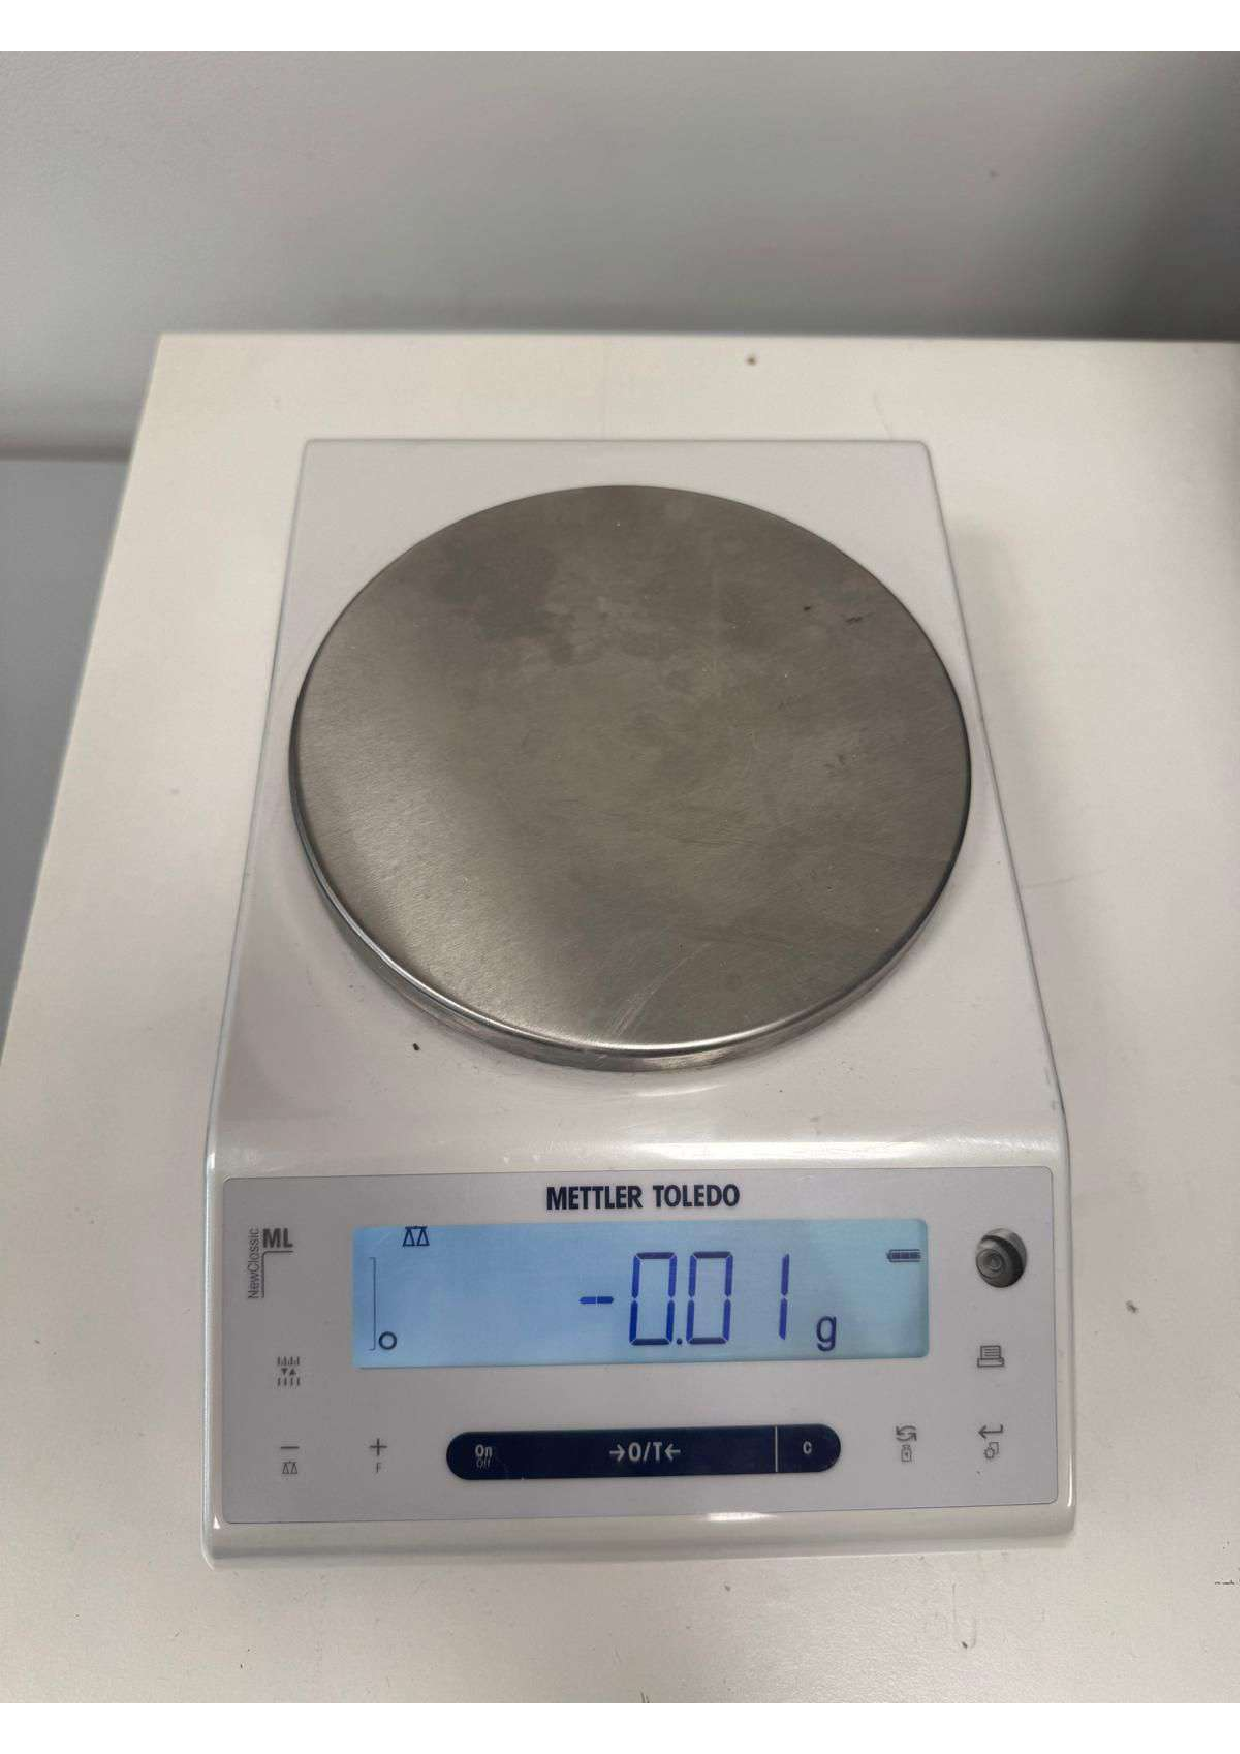
\includegraphics[width=0.5\textwidth]{WhatsApp Image 2024-10-25 at 16.42.23.pdf}
  \caption{Bilancia utilizzata in laboratorio}
\end{figure}

\section{Descrizione dei dati sperimentali}

\section{Analisi dei dati sperimentali}

\section{Conclusioni}
In conclusione il confronto tra le densità misurate e i valori di riferimento proposti ha fornito i seguenti risultati: 
Il cilindro 1 è composto di alluminio;
Il cilindro 2 è composto di ottone;
Il cilindro 3 è composto di plastica PVC;


\end{document}